\documentclass[11pt]{article}
\usepackage{mon_paquet}

\usepackage{marvosym}
\usepackage{mon_paquet}
\usepackage{amssymb}

\usepackage{hyperref}
\usepackage{comment}

\RequirePackage[left=1cm,right=1cm,top=1cm,bottom=1cm,noheadfoot]{geometry}
\RequirePackage{fancyhdr}\pagestyle{fancy}
\lhead{Formation Python}\rhead{Année Scolaire 2018-2019}\lfoot{}\rfoot{\LaTeXe{}}
\renewcommand\headrulewidth{0pt}%ligne en dessous de l'en tête


%graphes, physique-chimie
%\usepackage{pst-osci}\usepackage{pst-diffraction}\usepackage{pst-circ}\usepackage{pst-dosage}\usepackage{pst-labo}\usepackage{pst-optic}\usepackage{pst-spectra,pstricks-add}\usepackage[pictex]{m-ch-en}\usepackage{m-pictex,m-ch-en}
%\usepackage{psfrag}\usepackage{color,colortbl}\usepackage[table]{xcolor}\usepackage{graphicx}\usepackage[usenames,dvipsnames]{pstricks}\usepackage{epsfig}\usepackage{pst-grad}\usepackage{pst-plot}

%mise en page, multicolonnage, paysage, tableaux maths
%\usepackage{array}\usepackage{multirow}\usepackage{lscape}\usepackage{multido}

%paquets divers, maths, encadrement, symboles, cursif, qcm,lettrine,ombrage
%\usepackage{lettrine}\usepackage{eurosym}\usepackage{amsmath,amssymb,mathrsfs}\usepackage{esvect}\usepackage{esdiff}\usepackage{cancel}\usepackage{fancybox}\usepackage{shadow}\usepackage{pifont}\usepackage{fourier-orns}\usepackage{frcursive}\usepackage{bm}\usepackage{alterqcm}\usepackage{pstricks,pst-3d}(pour les ombres)\usepackage{enumitem}
%\renewcommand\thesection{\Roman{section}}
\usepackage{hyperref}\usepackage{esvect}\usepackage{bm}
\title{Formation Juin 2019 :\\$\star \star \star$\\Python pour l'enseignant de Physique-Chimie au lycée\\$\star \star \star$\\Bonus 2}\author{}\date{}
\begin{document}
\maketitle
\thispagestyle{fancy}





% Commandes de base
\newcommand{\from}[0]{\textcolor{orange}{from }}
\newcommand{\import}[0]{\textcolor{orange}{import }}
\newcommand{\for}[0]{\textcolor{orange}{for }}
\newcommand{\while}[0]{\textcolor{orange}{while }}
\newcommand{\dans}[0]{\textcolor{orange}{in }}
\newcommand{\si}[0]{\textcolor{orange}{if }}
\newcommand{\sinon}[0]{\textcolor{orange}{else }}
\newcommand{\True}[0]{\textcolor{orange}{True }}
\newcommand{\False}[0]{\textcolor{orange}{False }}
\renewcommand{\si}[0]{\textcolor{orange}{if }}
\renewcommand{\sinon}[0]{\textcolor{orange}{else }}
\newcommand{\et}[0]{\textcolor{orange}{and }}
\newcommand{\ou}[0]{\textcolor{orange}{or }}
\newcommand{\as}[0]{\textcolor{orange}{as }}
\newcommand{\defi}[0]{\textcolor{orange}{def }}
\newcommand{\return}[0]{\textcolor{orange}{return }}


\newcommand{\range}[0]{\textcolor{violet}{range}}
\newcommand{\chev}[0]{\textcolor{violet}{\scriptsize $\bm{>>>}$ }}
\newcommand{\print}[0]{\textcolor{violet}{print}}
\newcommand{\type}[0]{\textcolor{violet}{type}}
\newcommand{\dir}[0]{\textcolor{violet}{dir}}
\newcommand{\len}[0]{\textcolor{violet}{len}}
\renewcommand{\input}[0]{\textcolor{violet}{input}}
\newcommand{\float}[0]{\textcolor{violet}{float}}
%\renewcommand{\int}[0]{\textcolor{violet}{int}}
\newcommand{\abs}[0]{\textcolor{violet}{abs}}

\newcommand{\tab}[0]{\qquad \quad\,\, }
\newcommand{\tabis}[0]{\quad\, }


\newcommand{\str}[1]{\textcolor{green}{#1}}

\renewcommand{\com}[1]{\textcolor{red}{#1}}

%Environnement Python : 
 \newenvironment{python}[1]{\begin{center}\begin{normalsize}\begin{sffamily}
 \begin{minipage}{#1\textwidth}%
\hrulefill~\raisebox{-0.8ex}{{\Large \textcolor{red}{\Keyboard}} \quad\textcolor{red}{\textit{\textsf{code Python}}}\quad {\Large\textcolor{red}{\Keyboard}}}~\hrulefill\par}%
{\par\hrulefill \end{minipage}
\end{sffamily}\end{normalsize}\end{center}}




%Environnement correction Python : 
 \newenvironment{correc}[1]{\begin{center}\begin{normalsize}\begin{sffamily}
 \begin{minipage}{#1\textwidth}%
\hrulefill~\raisebox{-0.8ex}{{\Large \textcolor{red}{\Keyboard}} \quad\textcolor{red}{\textit{\textsf{\textsc{une correction possible}}}}\quad {\Large\textcolor{red}{\Keyboard}}}~\hrulefill\par}%
{\par\hrulefill \end{minipage}
\end{sffamily}\end{normalsize}\end{center}}

















% Autres : quasi pas utilisé depuis l'environnement Python
\newcommand{\ora}[1]{\textcolor{orange}{\texttt{#1}}}
\newcommand{\vio}[1]{\textcolor{violet}{\texttt{#1}}}
\newcommand{\rou}[1]{\textcolor{red}{\texttt{#1}}}




%%%%%%%%%%%%%%%%%%%%%%%%%%%%%%%%%%%%%%%%%%%%%%%%%%%%%%%%%%%%%%%%%%%%%%%%%%%%%%%%%%%%%%%%%%%%%%%%%%%%%%%%%%%%%%%%%%%%%%%%%%%%%%%%%%%%%%%%%%%%%%%%%%%%%%%%%%%%%%%%%%%%%%%%%%%%%%%%%%%%%%%%%%%%%%%%%%%%%%%%%%%%%%%%%%%%%%%%%%%%%%%%%%%%%%%%%%%%%%%%%%%%%%%%%%%%%%%%%%%%%%%%%%%%%%%%%%%%%%%%%%%%%%%%%%%%%%%%%%%%%%%%%%%%%%%%%%%%%%%%%%%%%%%%%%%%%%%%%%%%%%%%%%%%%%%%%%%%%%%%%%%%%%%%%%%%%%%%%%%%%%%%%%%%%%%%%%%%%%%%%%%%%%%%%%%%%


\vspace{-2.5cm}

\tableofcontents

\bigskip

\begin{itemize}

\item \textit{Le lien vers cet énoncé en ligne est sur le "padlet" (Bonus 2 formation); téléchargez-le et utilisez-le pour accéder aux liens cliquables de l'énoncé.}


\medskip

\textit{Vous pouvez aussi télécharger l'énoncé à cette adresse : }


\begin{center}
\underline{\url{https://github.com/formationPythonPC-Juin/enonce-donnees/blob/master/bonus2.pdf}                                                                                               }
\end{center}







\bigskip










\item \textit{Par rapport aux l'énoncés précédents, celui-ci ne propose pas  de fichiers d'aides.}

\medskip

\textit{Quoiqu'il en soit, les fichiers corrections sont donnés en lien à la fin de chaque partie.}

\medskip
\textit{Vous réalisez donc les exercices via le niveau 1 (pas d'aide) ou le niveau 3 (correction donnée, il vous faut alors commenter les lignes de code pour expliquer à quoi elles servent).} 








\bigskip














\end{itemize}


\begin{comment}




\item Tous \underline{les liens soulignés} du présent énoncé sont cliquables et permettent d'accéder aux tutoriels, à des fichiers aides ou aux fichiers corrections.

\item \textit{Vous aurez auprès de vous les documents mis à disposition sur le site académique et en premier lieu : }
\begin{itemize}
 \item \href{http://pedagogie.ac-limoges.fr/physique-chimie/IMG/pdf/python-trace_de_graphe.pdf}{\underline{\texttt{Tracés de graphes avec Python}}} signalé dans ce poly par: \textsc{vademecum}
 \item \href{http://pedagogie.ac-limoges.fr/physique-chimie/IMG/pdf/python-tutoriel.pdf}{\underline{\texttt{Tutoriel pour Python}}} signalé dans ce poly par: \textsc{tutoriel}
\end{itemize}

\medskip
\item \textit{Vous traitez les exercices dans l'ordre (difficulté croissante).}

\medskip
\item \textit{Pour chaque grande partie, vous créerez un fichier (stipulé dans l'énoncé).}

\medskip
\item \textit{Chaque partie peut se traiter selon 3 niveaux de difficulté :} 

\begin{itemize}
 \item \textbf{niveau 1} : on suit les questions dans l'ordre, en s'aidant ponctuellement des tutoriels et sans copier les codes proposés.
 \item \textbf{niveau 2} : dès le début de chaque exercice, des aides à la résolution sous forme de morceaux de code sont données ; on copie-colle ces codes dans les programmes et on les complète pour répondre aux questions posées
 \item \textbf{niveau 3} : on utilise les corrections données en fin de chaque partie. Le travail alors et de \textbf{commenter} les différentes lignes du programme, c'est à dire d'expliquer à quoi sert chaque ligne.
 
 \textsc{rappels : }
 \begin{itemize}
  \item les commentaires sont des éléments du programme qui ne sont pas lus par Python, mais qui sont présents pour aider l'utilisateur du programme
  \item les commentaires sur une ligne sont introduits par \# (apparaissent en rouge sous IDLE)
  \item les commentaires sur plusieurs lignes sont introduits et terminés par un triple guillemet : \textbf{"""} (apparaissent en vert sous IDLE)
 \end{itemize}
 
\end{itemize}


\medskip
\item À chacun de choisir son niveau de difficulté ; conseil : 

\begin{itemize}
 \item Par défaut, commencez par le niveau 2, c'est ainsi que l'énoncé est rédigé. 
 
 Si vous vous sentez à l'aise, vous pouvez tenter de réaliser les exercices sans les aides (niveau 1).
 
 Si vous avez des difficultés, passez au niveau 3.
\end{itemize}


\smallskip
\item \textit{Enfin, et même si cela n'est pas précisé, pensez à compiler votre code régulièrement pour vérifier si vous répondez bien aux questions.}

\end{itemize}



\end{comment}

%%%%%%%%%%%%%%%%%%%%%%%%%%%%%%%%%%%%%%%%%%%%%%%%%%%%%%%%%%%%%%%%%%%%
%%%%%%%%%%%%%%%%%%%%%%%%%%%%%%%%%%%%%%%%%%%%%%%%%%%%%%%%%%%%%%%%%%%%
%%%%%%%%%%%%%%%%%%%%%%%%%%%%%%%%%%%%%%%%%%%%%%%%%%%%%%%%%%%%%%%%%%%%
%%%%%%%%%%%%%%%%%%%%%%%%%%%%%%%%%%%%%%%%%%%%%%%%%%%%%%%%%%%%%%%%%%%%
%%%%%%%%%%%%%%%%%%%%%%%%%%%%%%%%%%%%%%%%%%%%%%%%%%%%%%%%%%%%%%%%%%%%





\newpage

\setcounter{section}{8}


\section{Résolutions numériques d'équations différentielles}




Au vu de ce qui est fait en classe de 2\textsuperscript{nde} et de 1\textsuperscript{ère}, on peut imaginer qu'en classe de Terminale (Spécialité), les élèves pourront rencontrer des équations différentielles. 

\smallskip
Python propose des méthodes pour approximer numériquement les solutions d'équations différentielles (ordre 1, 2 ou plus, linéaires ou non linéaires).

\smallskip
Donc, même sans connaître les solutions exactes dans des cas restreints (ordre 1 ou 2, linéaires et sans second membre), on peut "facilement" avoir une solution numérique grâce à la méthode \texttt{odeint()} du paquet \texttt{scipy.integrate}.

\smallskip
De plus, les modèles numériques permettent très rapidement d'implémenter des méthodes, encore il y a peu dans les programmes, telle la méthode d'Euler explicite.

\smallskip
Pour la suite, on s'intéressera à deux cas : 

\begin{itemize}
 \item chute libre avec frottements quadratiques : équation différentielle d'ordre 1 non linéaire ; l'équation est résolvable mais au prix de calculs relativement longs.
 \item pendule simple hors de l'approximation des petits angles : équation différentielle d'ordre 2 non linéaire ; pas de solution exacte. 
\end{itemize}




\smallskip
La suite de ce document se propose de voir ces deux cas à travers 3 méthodes de résolution numérique :  
\begin{itemize}
 \item la méthode d'Euler explicite
 \item la méthode d'Euler implicite
 \item l'utilisation d'une autre méthode numérique plus évoluée : la fonction \texttt{odeint()}.
\end{itemize}


\medskip

\textsc{remarque : } Dans l'hypothèse où les élèves de Terminale ne connaîtront pas les solutions classiques d'équations différentielles, il peut tout de même être intéressant d'utiliser les méthodes d'Euler ou la méthode \texttt{odeint} pour résoudre des cas classiques (chute libre sans frottement, avec frottements linéaires, pendule simple dans l'approximation des petits angles \ldots )



\medskip


Il faut noter qu'il existe encore de nombreuses méthodes de résolution numérique (on peut citer la méthode de Verlet, la méthode de Runge-Kutta, la méthode des éléments finis \ldots ).


\medskip
On étudie ici les méthodes les plus simples (méthodes d'Euler) ainsi qu'une méthode hybride fournie par Python (via la fonction \texttt{odeint}).






\subsection{Démonstrations générales pour les méthodes d'Euler}


On suppose une équation différentielle du type $\dfrac{dy}{dt} = f(t,y)$

\subsubsection{Première démonstration}

Avec celle-ci, on comprend bien le passage vers Euler explicite

\begin{itemize}
 \item discrétisation du temps : on coupe notre intervalle de temps avec un pas de temps $h$ ; les temps sont discrétisés : $t_0, t_1, t_2,\ldots t_n, t_{n+1}$
 \item on peut écrire (développement de Taylor) que $y(t_{n+1}) = y(t_n+h) = y(t_n)+h\times \dfrac{\text{d}y}{\text{d}t}(t_n) + \dfrac{h^2}{{2!}}\times \dfrac{\text{d}^2y}{\text{d}t^2}(t_n)+o(h^3)$
 \item Soit, si $h$ est assez petit : $y(t_{n+1}) \approx y(t_n)+h\times \dfrac{\text{d}y}{\text{d}t}(t_n)$
 \item Et finalement, \fbox{$\dfrac{\text{d}y}{\text{d}t}(t_n) \approx \dfrac{y(t_{n+1}) - y(t_n)}{h}$} où $h$ est le pas de temps.
\end{itemize}

$\Longrightarrow$ on remplacera toutes les dérivées par cette formule dans les méthodes d'Euler.



Soit : \fbox{$y(t_{n+1}) = y(t_n) + h\times f(t,y)$} :  \textbf{on a le schéma d'Euler explicite.}




Le problème c'est qu'on ne voit pas vraiment le schéma d'Euler implicite ; voilà une seconde démonstration pour le faire apparaître clairement.









\subsubsection{Seconde démonstration}

$\dfrac{dy}{dt} = f(t,y)$ : Intégrons cette équation entre $t_n$ et $t_{n+1}$ soit sur l'intervalle $h$ : 

$\displaystyle \int _{t_n}^{t_{n+1}} \dfrac{dy}{dt}\cdot dt = \int _{t_n}^{t_{n+1}} f(t,y)\cdot dt$
soit $y(t_{n+1}) - y(t_n) = \displaystyle \int _{t_n}^{t_{n+1}} f(t,y)\cdot dt$


\smallskip

\newpage

\begin{multicols}{2}
Le second membre pose problème, elle représente l'aire sous la courbe de la fonction $f$ : 

D'après le schéma ci-contre, on peut approximer cette aire de deux façons : 



soit en la minorant (si $f$ est croissante) et dans ce cas, l'aire sera : $h\times f(t_n, y(t_n))$ $\Longrightarrow$ \textbf{Euler explicite}

soit en la majorant (si $f$ est croissante), et dans ce cas, l'aire sera : $h\times f(t_{n+1}, y(t_{n+1}))$ $\Longrightarrow$ \textbf{Euler implicite}

\psscalebox{1.0 1.0} % Change this value to rescale the drawing.
{
\begin{pspicture}(0,-2.3959303)(7.54,2.3959303)
\psline[linecolor=black, linewidth=0.04, arrowsize=0.05291667cm 2.0,arrowlength=1.4,arrowinset=0.0]{->}(3.2,-1.511028)(3.2,2.088972)(3.2,2.488972)
\psline[linecolor=black, linewidth=0.04, arrowsize=0.05291667cm 2.0,arrowlength=1.4,arrowinset=0.0]{->}(2.8,-1.511028)(7.2,-1.511028)
\psbezier[linecolor=black, linewidth=0.04](3.6,-0.711028)(4.0,0.888972)(6.4,2.888972)(7.2,1.6889720052083335)
\psline[linecolor=black, linewidth=0.04, linestyle=dotted, dotsep=0.10583334cm](4.0,0.088972)(4.0,-1.511028)
\psline[linecolor=black, linewidth=0.04, linestyle=dotted, dotsep=0.10583334cm](6.4,2.088972)(6.4,-1.511028)
\psline[linecolor=black, linewidth=0.04, linestyle=dotted, dotsep=0.10583334cm](4.0,0.088972)(3.2,0.088972)
\psline[linecolor=black, linewidth=0.04, linestyle=dotted, dotsep=0.10583334cm](6.4,2.088972)(3.2,2.088972)
\rput[bl](3.6,-1.911028){$t_n$}
\rput[bl](5.8,-1.911028){$t_{n+1}$}
\rput[bl](4.8,-2.311028){$h$}
\rput[bl](1.2,0.088972){$f(t_n, y(t_n))$}
\rput[bl](0.4,2.00){$f(t_{n+1}, y(t_{n+1}))$}
\psline[linecolor=black, linewidth=0.04, linestyle=dashed, dash=0.17638889cm 0.10583334cm](4.0,0.088972)(6.4,0.088972)
\psline[linecolor=black, linewidth=0.04, linestyle=dashed, dash=0.17638889cm 0.10583334cm](4.0,2.088972)(4.0,0.088972)
\end{pspicture}
}

\end{multicols}






\subsubsection{Euler explicite}


Reprenons notre équation de départ : 

$\frac{dy}{dt} = f(t,y)$

Avec la méthode d'Euler explicite, on se base sur le comportement de dérivée, position\ldots au point $n$ : 

$\dfrac{\text{d}y}{\text{d}t}(t_n) \approx \dfrac{y(t_{n+1}) - y(t_n)}{h} \approx f(t_n , y(t_n))$




\subsubsection{Euler implicite}


Reprenons notre équation de départ : 

$\frac{dy}{dt} = f(t,y)$

Avec la méthode d'Euler implicite, on se base sur le comportement de dérivée, position\ldots au point $n+1$ : 

$\dfrac{\text{d}y}{\text{d}t}(t_n) \approx \dfrac{y(t_{n+1}) - y(t_n)}{h} \approx f(t_{n+1} , y(t_{n+1}))$




\begin{center}
\textbf{Euler implicite diverge généralement moins qu'Euler explicite.}                                                                       \end{center}







\subsection{Utilisation de la fonction \texttt{odeint()}}


Celle ci est utilisable via l'importation du paquet \texttt{scipy.integrate} : 

\from scipy.integrate \import odeint


Le principe consiste  : 
\begin{enumerate}


\item à donner l'équation différentielle à Python, sous la forme d'une définition de fonction.

\item Puis de définir l'intervalle de temps et le pas de temps utilisé pour réaliser l'approximation de la solution.

\item De définir bien sûr les conditions initiales.

\item D'enfin faire appel à la méthode \texttt{odeint()} pour résoudre l'équation ; les paramètres donnés à cette fonction étant l'équation différentielle (1), les CI (3), le tableau de temps utile à la résolution (2).

\end{enumerate}


Nous verrons cette méthode à travers les exemples.










\subsection{Chute libre avec frottements quadratiques}

Dans ce cas-là (frottements proportionnels à $v^2$, la solution exacte est longue à trouver. Le recours à des solutions numériques peut être envisagé.

La force de frottement peut se mettre sous la forme : $\vv{F} = -f\times v^2\cdot \dfrac{\vv{v}}{|v|}$ 


L'équation différentielle donne : 

$\left\{\begin{array}{ll}
 m\cdot \frac{\text{d}{v}}{\text{d}t} =& -f\cdot {v}^2+m\cdot{g}\\
 
 \vv{v} =& \frac{\text{d}\vv{r}}{\text{d}t}
 
\end{array}\right.$ soit en projection sur l'axe : 
$\left\{\begin{array}{ll}
 m\cdot \frac{\text{d}{v}}{\text{d}t} =& -f\cdot {v}^2+m\cdot {g}\quad (1)\\
 
 {v} =& \frac{\text{d}{y}}{\text{d}t} \quad (2)
 
\end{array}\right.$

Dans ce cas, on constate que les variables $y$ et $v$ ne sont pas liées, ce qui va nous simplifier la tâche.

Les CI sont $v(t = 0) = 0$ et $y(t = 0) = 0$.

\smallskip
Les valeurs des grandeurs entrant en jeu : 
\begin{itemize}
 \item $m = 80\;\text{kg}$
 \item $f = 0,17 \;\text{SI}$
 \item $g = 9,81\;\text{SI}$
 \item L'axe $Oy$ est choisi positif vers le bas
\end{itemize}



\medskip

\subsubsection{Méthode d'Euler explicite}

Il suffit de traduire la dérivée par le taux d'accroissement entre 2 instants proches séparés de $h$ : 

$m\cdot \frac{\text{d}{v}}{\text{d}t} \approx m\cdot \dfrac{v_{n+1} - v_n}{h} \approx -f\cdot {v_n}^2+m\cdot{g}$



Soit encore : \fbox{$v_{n+1} = v_n -\dfrac{h}{m}\times (f\cdot {v_n}^2-m\cdot{g})$} avec $h$ le pas de temps, $h = dt$


De la seconde équation, on tire \fbox{$y_{n+1}=y_n+h\times v$} avec $h$ le pas de temps, $h = dt$



Ce sont ces deux équations qu'il va nous falloir traduire dans notre programme, en tenant compte des C.I.


\smallskip

Vous pourrez créer un programme \texttt{chute-euler-explicite.py}.

\smallskip


\begin{enumerate}
 \item Donner les valeurs des grandeurs entrant en jeu dans l'étude dans des variables aux noms explicites.
 \item De même, intégrer vos conditions initiales à votre programme. Par la même occasion, on fixera un temps initial $t=0$ et un pas de temps pour les calculs d'une seconde : $dt = 1$ ou $h = 1$ selon vos notations.
 \item Entrez alors les formules des forces intervenant : poids et frottements.
 \item Initialisez des listes vides pour la position (Y1), la vitesse (V1) et le temps (T1).
 \item Créez alors une boucle qui permet sur les 30 premières secondes de chute libre de : 
 \begin{itemize}
  \item implémenter vos listes Y1, V1 et T1 des valeurs de $y$, $v$ et $t$ au moment considéré
  \item calculer à nouveau la force de frottements, le poids et la somme des forces
  \item en déduire la nouvelle position en fonction de la précédente
  \item en déduire la nouvelle vitesse en fonction de la précédente
  \item vous n'oublierez pas d'augmenter alors le temps actuel du pas de temps choisi ($dt$ ou $h$)
 \end{itemize}
\item Représentez dès lors la vitesse de l'objet en fonction du temps.
\end{enumerate}





\begin{center}
$\blacktriangleright$ \href{https://github.com/formationPythonPC-Juin/corrections-formation/blob/master/chute-euler-explicite.py}{\underline{\texttt{lien vers la correction de cet exercice : chute-euler-explicite.py}}}$\blacktriangleleft$                                                                                                                                                                    \end{center}











\subsubsection{Méthode d'Euler implicite}

L'idée est la même sauf que cette fois-ci : 

 $m\cdot \frac{\text{d}{v}}{\text{d}t} \approx m\cdot \dfrac{v_{n+1} - v_n}{h} \approx -f\cdot {v_{n+1}}^2+m\cdot {g}$.

\smallskip
L'ensemble est moins trivial car on voit se dessiner un polynôme de degré 2 en $v_{n+1}$. 

\smallskip
On cherche son discriminant et la solution positive en $v_{n+1}$ qui nous donne : 

$v_{n+1} = \dfrac{-1+\sqrt{1+4\times (f\cdot h/m)\cdot (v_n +h\cdot g)}}{2\cdot (f\cdot h/m)}$
 
 
 
 

\smallskip

Vous pourrez créer un programme \texttt{chute-euler-implicite.py}.

\smallskip


 
 
 

 $\Longrightarrow$ Se servir de cette formule pour implémenter un code fournissant la représentation de la solution (vitesse en fonction du temps) de l'équation différentielle par la méthode Euler implicite (il n'y a quasiment rien à changer par rapport au code précédent).
 
 
 


\begin{center}
$\blacktriangleright$ \href{https://github.com/formationPythonPC-Juin/corrections-formation/blob/master/chute-euler-implicite.py}{\underline{\texttt{lien vers la correction de cet exercice : chute-euler-implicite.py}}}$\blacktriangleleft$                                                                                                                                                                    \end{center}


 
 
 
 
 
 
 \subsubsection{Méthode \texttt{odeint()} du paquet \texttt{scipy.integrate}}
 
 La méthode \texttt{odeint()} fournit une résolution numérique plus précise que les deux méthodes vues précédemment.
 
 \smallskip
 
 

Vous pourrez créer un programme \texttt{chute-odeint.py}.

\smallskip


 
 $\Longrightarrow$ Interprétez chaque ligne \href{https://github.com/formationPythonPC-Juin/corrections-formation/blob/master/chute-odeint.py}{\underline{du code fourni ici (\texttt{chute-odeint.py})}} ; tâchez de comprendre à partir de ce dernier comment fonctionne la méthode odeint.
 
 
 
 
 
 
 
 \subsubsection{Comparaison des trois méthodes}
 
 
 $\Longrightarrow$ Sur un même graphe, représentez les solutions (vitesse en fonction du temps) du problème de la chute libre avec frottements quadratiques par les méthodes d'Euler explicite, Euler implicite et par la méthode odeint.
  
  
  
  

\smallskip

Vous pourrez créer un programme \texttt{chute-3methodes.py}.

\smallskip


 
\begin{center}
$\blacktriangleright$ \href{https://github.com/formationPythonPC/corrections-formation/blob/master/chute-3methodes.py}{\underline{\texttt{lien vers la correction de cet exercice : chute-3methodes.py}}}$\blacktriangleleft$                                                                                                                                                                    \end{center}

 
 
 
 
 
 %%%%%%%%%%%%%%%%%%%%%%%%%%%%%%%%%%%%%%%%%%%%%%%%%%%%%%%%%%%%%%%%%%%%%%%%%%%%%%%%%%%%%%%%%%%%%%%
 %%%%%%%%%%%%%%%%%%%%%%%%%%%%%%%%%%%%%%%%%%%%%%%%%%%%%%%%%%%%%%%%%%%%%%%%%%%%%%%%%%%%%%%%%%%%%%%
  %%%%%%%%%%%%%%%%%%%%%%%%%%%%%%%%%%%%%%%%%%%%%%%%%%%%%%%%%%%%%%%%%%%%%%%%%%%%%%%%%%%%%%%%%%%%%%%
   %%%%%%%%%%%%%%%%%%%%%%%%%%%%%%%%%%%%%%%%%%%%%%%%%%%%%%%%%%%%%%%%%%%%%%%%%%%%%%%%%%%%%%%%%%%%%%%
    %%%%%%%%%%%%%%%%%%%%%%%%%%%%%%%%%%%%%%%%%%%%%%%%%%%%%%%%%%%%%%%%%%%%%%%%%%%%%%%%%%%%%%%%%%%%%%%
    
 
 
 
 
 
 
 
 \subsection{Pendule simple en dehors de l'approximation des petits angles}
 
 L'équation différentielle du mouvement est : $\dfrac{\text{d}^2\theta}{\text{d}t^2} = -\dfrac{g}{\ell}\cdot \sin \theta$. On ne connaît pas de solution exacte pour cette situation.


Posons $\omega_0^2 = \dfrac{g}{\ell}$ alors $\ddot{\theta} = -\omega_0^2\cdot \sin \theta$ où $\theta$ représente l'angle entre la verticale et l'axe du pendule, $\ell$ la longueur du fil, $g$ l'accélération de la pesanteur.

 
 \subsubsection{Rappels mathématiques}
 
 Comme on a pu s'en rendre compte, les méthodes employées jusqu'ici ne concernent que des équations différentielles d'ordre 1.
 
 \smallskip
 
 Dès lors, une question se pose : Comment gérer des équations différentielles d'ordre supérieur ?
 
 \smallskip
 
 Les mathématiques nous apprennent que toute équation différentielle d'ordre $n$ peut se mettre sous la forme de $n$ équations différentielles d'ordre 1 ; on pourra résoudre toutes ces équations par les méthodes vues plus haut.
 
 \smallskip
 
 La conséquence indirecte et malheureuse de cela est qu'en cherchant à diminuer l'ordre de l'équation différentielle, on va créer des inconnues matricielles (vectorielles) comme on va le voir dans le cas du pendule simple (on diminue l'ordre des équations différentielles mais on augmente la dimension de l'espace des fonctions solutions).
 
 
 \subsubsection{Mise en équation dans le cas du pendule simple}
 

On pose $\Omega = \dot{\theta}$ (pulsation) et on  crée une variable vectorielle : $X = \left(\begin{array}{l}
                                                     \theta\\
                                                     \Omega
                                                    \end{array}\right)$

et on obtient alors l'équation différentielle suivante : 

$\dot{X} = \left(\begin{array}{l}
                                                     \dot{\theta}\\
                                                     \ddot{\theta}
                                                    \end{array}\right) = \left(\begin{array}{c}
                                                     \Omega\\
                                                     -\omega_0^2\cdot \sin \theta
                                                    \end{array}\right)$

                                                    soit $\dot{X} = \left(\begin{array}{c}
                                                     X[1]\\
                                                     -\omega_0^2\cdot \sin X[0]
                                                    \end{array}\right)$


Comme on le constate dans cet exemple, nous nous sommes ramenés à 2 équations différentielles d'ordre 1 dans lesquelles les variables sont \underline{couplées}. On a diminué l'ordre (ordre 1) mais on s'est alors ramené à des inconnues matricielles (vectorielles) et non plus scalaires.

  
  \medskip

  Pour la suite on considère un pendule simple avec : 
  \begin{itemize}
   \item $\ell = 0,25\;\text{m}$
   \item $g = 10\;\text{m.s}^{-2}$
   \item $\theta(t=0) = 0$
   \item $\dot{\theta}(t=0) = \Omega(t=0) = 2\;\text{rad.s}^{-1}$
  \end{itemize}

  \smallskip
  
    On limite l'étude aux 8 premières secondes d'évolution. On choisira un pas de temps $dt = 0,02\;\text{s}$ pour toutes les méthodes.
    
\smallskip

On cherche à représenter la pulsation en fonction du temps par les 3 méthodes vues plus haut.




\subsubsection{Méthode d'Euler explicite}


Vous pouvez créer un programme \texttt{pendule-euler-explicite.py}

\smallskip


L'équation différentielle vectorielle ci-dessus se traduit en approximant le développement de Taylor à l'ordre 1 par :

\begin{itemize}
 \item $\theta_{n+1} - \theta_n = \Omega_n\times dt \Longrightarrow \theta_{n+1} = \theta_n + \Omega_n\times dt $
 \item  $\Omega_{n+1} - \Omega_n = -\omega_0^2\cdot dt\cdot \sin \theta_n \Longrightarrow \Omega_{n+1} = \Omega_n -\omega_0^2\cdot dt\cdot \sin \theta_n$
\end{itemize}




\begin{enumerate}
 \item Définir les constantes et les C.I.
 \item Définir de même 3 listes vides \texttt{angle1}, \texttt{puls1} et \texttt{T1} vides qui contiendront les valeurs d'angles, de pulsations et de temps au cours du mouvement.
 \item Créez une boucle pour les 10 premières secondes d'évolution au sein de laquelle : 
 \begin{itemize}
  \item vous implémentez les 3 listes créées vides précédemment
  \item vous traduisez les deux équations vues précédemment
  \item vous n'oublierez pas d'incrémenter le temps en fin de boucle
 \end{itemize}

 \item Représentez l'évolution de la pulsation au cours de ces 10 premières secondes ; conclusions.
\end{enumerate}




 
\begin{center}
$\blacktriangleright$ \href{https://github.com/formationPythonPC-Juin/corrections-formation/blob/master/pendule-euler-explicite.py}{\underline{\texttt{lien vers la correction de cet exercice : pendule-euler-explicite.py}}}$\blacktriangleleft$                                                                                                                                                                    \end{center}

 


 
 
 
 
 
\subsubsection{Méthode d'Euler implicite}


Vous pouvez créer un programme \texttt{pendule-euler-implicite.py}

\smallskip

La solution précédente diverge totalement ; on va essayer de stabiliser les solutions en modifiant la référence à l'angle dans le calcul de la pulsation : 

\begin{itemize}
 \item $\theta_{n+1} = \theta_n + \Omega_n\times dt $
 \item $\Omega_{n+1} = \Omega_n -\omega_0^2\cdot dt\cdot \sin \theta_{n+1}$
\end{itemize}


L'ordre des calculs est ici essentiel, puisqu'on a besoin de la première équation pour résoudre la seconde.

\medskip

 $\Longrightarrow$ Se servir de ces formules pour implémenter un code fournissant la représentation de la solution (pulsation en fonction du temps) de l'équation différentielle par la méthode Euler implicite (il n'y a quasiment rien à changer par rapport au code précédent).
 
 
 


\begin{center}
$\blacktriangleright$ \href{https://github.com/formationPythonPC-Juin/corrections-formation/blob/master/pendule-euler-implicite.py}{\underline{\texttt{lien vers la correction de cet exercice : pendule-euler-implicite.py}}}$\blacktriangleleft$                                                                                                                                                                    \end{center}


 





 
 
 
 
 
 

 
 
 
 \subsubsection{Méthode \texttt{odeint()} du paquet \texttt{scipy.integrate}}
 
 La méthode \texttt{odeint()} fournit une résolution numérique plus précise que les deux méthodes vus précédemment.
 
 \smallskip
 
 

Vous pourrez créer un programme \texttt{pendule-odeint.py}.

\smallskip


 
 $\Longrightarrow$ Trouvez par la méthode \texttt{odeint()} la représentation graphique de la pulsation en fonction du temps au cours des 10 premières secondes d'évolution.
 
 
 \smallskip
 
 \textsc{aide : }
 
 Ici, il faudra choisir pour résoudre l'équation différentielle par \texttt{odeint()} une inconnue vectorielle qu'on a notée $X$ plus haut. 
 
 D'après la définition de $X$, il faudra ensuite représenter $X[1]$ en fonction du temps.
 

 
 
 
 
 

\begin{center}
$\blacktriangleright$ \href{https://github.com/formationPythonPC-Juin/corrections-formation/blob/master/pendule-odeint.py}{\underline{\texttt{lien vers la correction de cet exercice : pendule-odeint.py}}}$\blacktriangleleft$                                                                                                                                                                    \end{center}


 
 
 
 

 
 
 \subsubsection{Comparaison des trois méthodes}
 
 
 $\Longrightarrow$ Sur un même graphe, représentez les solutions (pulsation en fonction du temps) du problème du pendule simple par les méthodes d'Euler explicite, Euler implicite et par la méthode odeint.
  
  
  
  

\smallskip

Vous pourrez créer un programme \texttt{pendule-3methodes.py}.

\smallskip


 
\begin{center}
$\blacktriangleright$ \href{https://github.com/formationPythonPC-Juin/corrections-formation/blob/master/pendule-3methodes.py}{\underline{\texttt{lien vers la correction de cet exercice : pendule-3methodes.py}}}$\blacktriangleleft$                                                                                                                                                                    \end{center}

 
  
 
 
 
 %%%%%%%%%%%%%%%%%%%%%%%%%%%%%%%%%%%%%%%%%%%%%%%%%%%%%%%%%%%%%%%%%%%%%%%%%%%%%%%%%%%%%%%%%%%%%%%%%%%%%%%%%%%%%%%%%%%%%%%%%%%%%%%%%%%%%%%%%%%%%%%%%%%%%%%%%%%%%%%%%%%%%%%%%%%%%%%%%%%%%%%%%%%%%%%%%%%%%%%%%%%%%%%%%%%%%%%%%%%%%%%%%%%%%%%%%%%%%%%%%%%%%%%%%%%%%%%%%%%%%%%%%%%%%%%%%%%%%%%%%%%%%%%%%%%%%%%%%%%%%%%%%%%%%%%%%%%%%%%%%%%%%%%%%%%%%%%%%%%%%%%%%%%%%%%%%%%%%%%%%%%%%%%%%%%%%%%%%%%%%%%%%%%%%%%%%%%%%%%%%%%%%%%%%%%%%%%%%%%%%%%%%%%%%%%%%%%%%%%%%%%%%%%%%%%%%%%%%%%%%%%%%%%%%%%%%%%%%%%%%%%%%%%%%%%%%%%%%%%%%%%%%%%%%%%%%%%%%%%%%%%%%%%%%%%%%%%%%%%%%%%%%%%%%%%%%%%%%%%%%%%%%%%%%%%%%%%%%%%%%%%%%%%%%%%%%%%%%%%%%%%%%%%%%%%%%%%%%%%%%%%%%%%%%%%%%%%%%%%%%%%%%%%%%%%%%%%%%%
 
 




 
 \newpage
 
 \section{Communication Python $\longleftrightarrow$ microcontrôleurs}
 
 
 Quand on souhaite faire des acquisitions via un capteur en utilisant un microcontrôleur (Arduino\textsuperscript{TM}, MicroPython, \ldots), on est souvent tenté de vouloir enregistrer les données d'acquisitions. 
 
 Deux cas peuvent se présenter alors : 
 \begin{itemize}
  \item Votre microcontrôleur dispose d'une mémoire suffisante pour enregistrer les données ; dans ce cas, pas de problème.
  \item Votre microcontrôleur dispose de très peu d'espace mémoire (carte micro~:bit) ou ne dispose pas de mémoire de stockage du tout (Arduino\textsuperscript{TM}) et dans ce cas : comment fait-on ?
 \end{itemize}

 \subsection{La méthode de base}
 
 \subsubsection{Présentation}
 
 Les logiciels utilisés pour programmer votre microcontrôleur (IDE pour Arduino\textsuperscript{TM}, Mu-Editor pour microPython, Programming Editor pour PICAXE \ldots) vont vous permettre de communiquer avec la carte.
 
 \smallskip
 Ces logiciels vont permettre de communiquer avec la carte dans les deux sens via le \textbf{port série} reliant l'ordinateur au microcontrôleur et généralement "symbolisé" par un câble USB.
 
 \smallskip
 Le sens ordinateur $\rightarrow$ microcontrôleur est essentiel puisqu'il va permettre de programmer la carte.
 
 \medskip
 Mais l'autre sens existe aussi : on peut faire passer des informations du microcontrôleur à l'ordinateur via le port série.
 
 \medskip
 Ces logiciels disposent donc d'\textbf{une interface} permettant de voir ce qu'envoie le microcontrôleur. On lui donne le nom de moniteur série sous Arduino\textsuperscript{TM}, REPL dans les déclinaisons microPython, terminal Série chez PICAXE\ldots.
 
 
 
 
 
 
 
 
 
 
 \subsubsection{Cas pratique sous l'IDE Arduino\textsuperscript{TM}}
 
 Nous souhaitons acquérir les valeurs analogiques renvoyées par une carte microcontrôleur lors de la manipulation d'un potentiomètre. 
 

 
 \begin{center}
  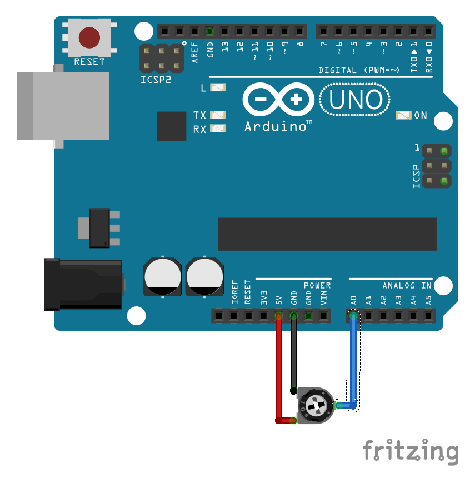
\includegraphics[scale=0.9]{potar.EPS}
 \end{center}
 
 
 Le potentiomètre est alimenté ici entre 0 et 5 Volts, et la broche centrale est placée sur une entrée analogique de la carte (ici A0 pour le microcontrôleur utilisé).
 
 \smallskip
 Le microcontrôleur transformera cette tension analogique en valeur numérique qu'on note \texttt{valeur} (entre 0 et 1023).
 
 \smallskip
 On souhaite voir afficher les valeurs que retourne le microcontrôleur sur l'interface série de l'ordinateur toutes les 500 ms. 
 
 \smallskip
 Un code possible pourrait être : 
 
 
 \begin{multicols}{2}
\begin{center}
  \textbf{Sous l'IDE Arduino :}                                 \end{center}
  
  Le premier bloc est un bloc de réglages, il n'est lu qu'une fois par Arduino ; on définit la broche A0 comme une entrée (de toute façon elle ne peut être autre chose), et puis surtout on définit la vitesse de communication avec le port série à 9600 bauds.
  
  On constate ici, comme en Python qu'on utilise une bibliothèque appelée Serial. Cette bibliothèque est importée d'office par Arduino\textsuperscript{TM}, nous n'avons pas eu à le faire dans le préambule.
  
  
  
  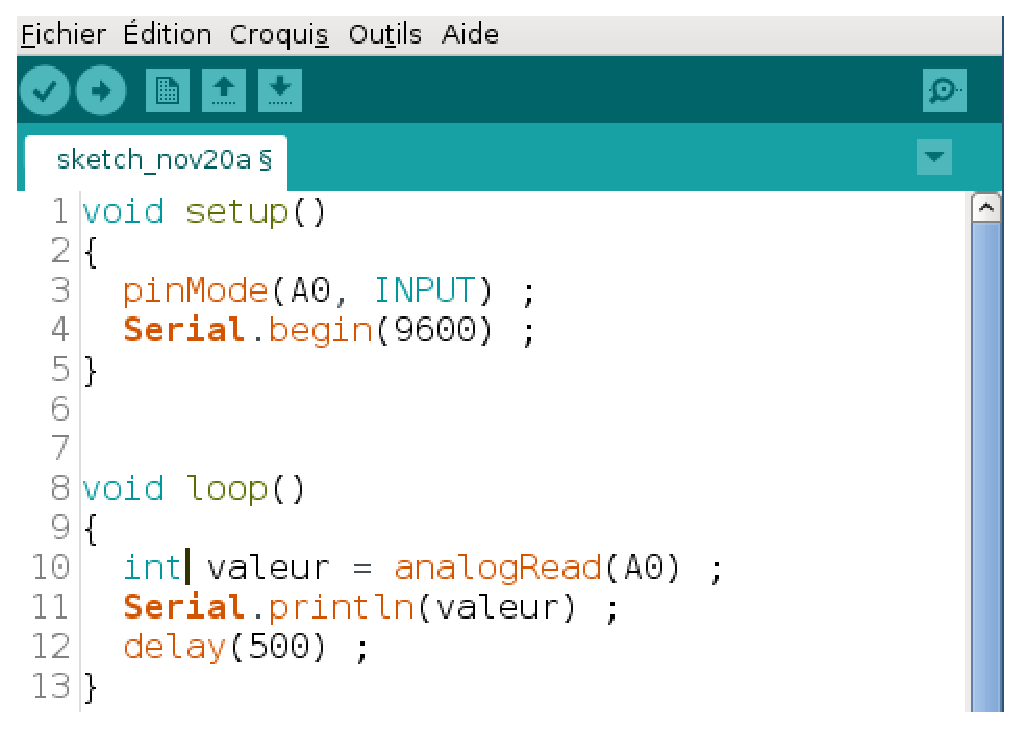
\includegraphics[scale=0.45]{arduino.EPS}
  
  
  
  \medskip
  Puis on rentre dans une boucle infinie (loop). 
  
  On définit tout d'abord une variable \texttt{valeur} comme un décimal (float) et qui vaut la valeur analogique lue sur la broche A0 ; donc l'image de la tension au centre du pont diviseur du potentiomètre.
  
  \smallskip
  Puis on refait appel à la bibliothèque Serial pour afficher (print) cette variable à travers le port série.
  
  \medskip
  Il suffit alors d'envoyer le code sur la carte puis d'ouvrir le moniteur série (avec la petite loupe en haut à droite) et s'affichent toutes les 500 ms les valeurs analogiques correspondant à la tension au centre du pont diviseur.
  
 \end{multicols}

 
 
 Quand on a assez de mesures, il suffit alors de faire un copier-coller vers un fichier, qu'on pourrait appeler \texttt{donnees.csv} et faire ensuite un traitement par tableur ou par Python comme en 1.5 page 3.
 
 
 
 
 
 
 
 \subsubsection{Cas pratique sous Mu-Editor pour microPython (carte micro~:bit)}
 
 
  
  \begin{center}
   \includegraphics[scale = 0.3]{microbit.EPS}
  \end{center}
  
  
  Cette fois-ci, la tension délivrée par la carte vaut 3,3 Volts. Les branchements sont là encore basiques. L'entrée notée 0 peut être une entrée numérique ou analogique.

  
  \smallskip
 Le microcontrôleur transformera la tension analogique lue sur l'entrée 0 en valeur numérique qu'on note \texttt{valeur} (entre 0 et 1023).
 
 \smallskip
 On souhaite voir afficher les valeurs que retourne le microcontrôleur sur l'interface série de l'ordinateur toutes les 500 ms. 
 
 \smallskip
 Un code possible pourrait être : 
 
 
 \begin{multicols}{2}
\begin{center}
  \textbf{Sous Mu-Editor :}                                 \end{center}
  
  
  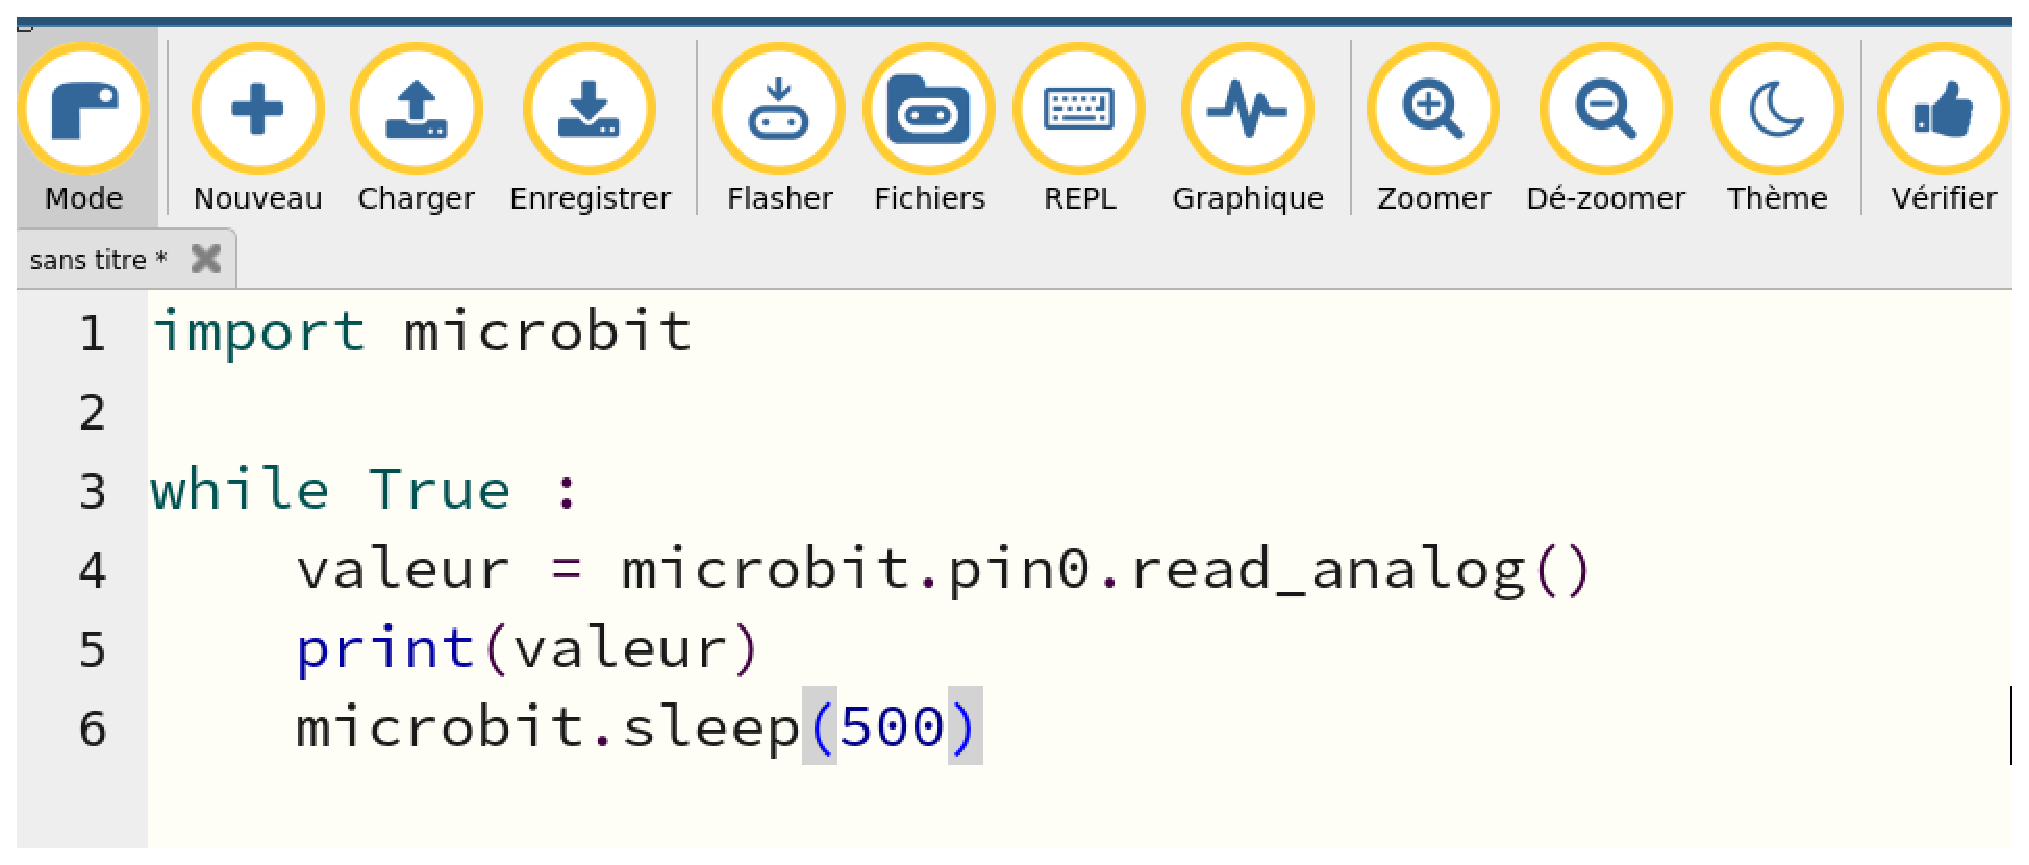
\includegraphics[scale = 0.25]{mu.EPS}
  
  
  
  On importe tout d'abord la bibliothèque microbit qui contient quasiment toutes les modules utiles pour faire fonctionner la carte ; cette bibliothèque est spécifique à cette carte.
  
  
  Puis on rentre dans une boucle infinie (while True) ; on définit alors une variable \texttt{valeur} par l'appel de la fonction \texttt{read\_analog} de la broche 0 gérée par le module \texttt{pin0} de la bibliothèque microbit.
  
  On affiche cette valeur. (Ici, pas d'appel à une bibliothèque Serial ; microPython "cache" la manipulation, et pourtant, les données vont bien voyager à travers le port série.
  
  Puis on fait une pause de 500 ms grâce à la fonction sleep de la bibliothèque microbit.
  
  Et la boucle infinie recommence.
  
  
  \medskip
  Il suffit alors d'envoyer le code sur la carte puis d'ouvrir le REPL (icône au dessus), de relancer la carte et s'affichent toutes les 500 ms les valeurs analogiques correspondant à la tension au centre du pont diviseur.
  
 \end{multicols}

 
 
 
 Quand on a assez de mesures là encore, il suffit alors de faire un copier-coller vers un fichier, qu'on pourrait appeler \texttt{donnees.csv} et faire ensuite un traitement par tableur ou par Python comme en 1.5 page 3.
 
 
 \medskip
 
 
 \textit{Des microcontrôleurs sont à votre disposition si vous désirez tester ces manipulations}
 
 
 
 
 
 
 
 
 
 
 
 
 
 \subsection{Le microcontrôleur communique avec Python (sur l'ordinateur)}
 
 Il existe une autre méthode, plus compliquée mais aussi beaucoup plus puissante. En fait Python (de votre ordinateur) est capable de communiquer avec un microcontrôleur dans les deux sens. Il peut : 
 
 \smallskip
 
 \begin{itemize}
  \item \textbf{commander un microcontrôleur} : par exemple, une acquisition est lancée via le microcontrôleur quand l'utilisateur le décide. (Ce cas-là bien que très intéressant pour des manipulations où on ne souhaite pas toucher à la carte ni au programme implanté dessus, ne sera pas étudié car il varie selon la carte utilisée et fait appel à des fonctions parfois "exotiques" propres à chaque microcontrôleur).
  \item  \textbf{Recevoir directement des informations d'un microcontrôleur} : dans ce cas-là, tout est automatique, et Python peut avec uniquement un seul programme, récupérer les données envoyées sur le port série, les enregistrer dans un fichier, les traiter pour représenter des graphes\ldots
 \end{itemize}

 \smallskip
 
 C'est ce deuxième cas que nous allons étudier. Il permet déjà de prendre conscience de la puissance de Python pour gérer des situations courantes dans notre discipline.
 
 
 
 \subsubsection{Compléments quant aux communications entre Python et les entrées / sorties}
 
 Pour gérer la communication avec le port série, Python dispose de la bibliothèque \texttt{pyserial} appelée par \texttt{import serial}. 
 
 
 \medskip
 Une première chose à savoir est que Python possède 2  "types" pour les chaînes de caractères : 
 \begin{itemize}
  \item le "type" \texttt{str} ou \texttt{string} qui est présenté sur le tuto disponible sur le site académique
  \item le "type" \texttt{byte} (octet) qui traite les séquences d'octets ; les chaînes de caractères sont des suites d'octets ; Python les traduit lors d'affichage écran par des caractères à peu près compréhensibles par l'utilisateur.
 \end{itemize}

 \medskip
$\Longrightarrow$ Quand vous utilisez un programme Python, tout ce qui rentre ou sort de votre programme est typé "\texttt{bytes}".
 
 \medskip
 
 
 Cela signifie que si Python arrive à lire des données provenant par exemple du port série de l'ordinateur, elles seront de type \texttt{bytes} et il faudra donc pouvoir les transformer en format lisible (\texttt{string}) : cela se fait par la méthode \texttt{.decode("utf8")} ; l'utf-8 étant l'encodage utilisé par Python3.
 
 
 \subsubsection{Notre objectif}
 
 
 \begin{itemize}
  \item Un microcontrôleur envoie des données sur le port série ; ces données ne sont pas lues par le moniteur série (Arduino\textsuperscript{TM}) le REPL (MicroPython), le terminal série (PICAXE)\ldots
  
  \item Il est essentiel dans cette hypothèse de ne pas ouvrir l' interface série, sinon il y a conflit entre Python et cette interface.
  \item Nous souhaitons que notre programme Python puisse récupérer les données en provenance de la carte et les copie dans un fichier \texttt{donnees.csv}.
  \item Les codes utilisés pour les microcontrôleurs sont les mêmes que précédemment : on souhaite donc enregistrer la valeur lue par l'entrée analogique de la carte dans un fichier par l'intermédiaire de Python.
  \item Pour ce qui suit, la carte est déjà programmée par les codes vus précédemment ; elle fait son travail : elle envoie les données sur le port série ; voyons à présent comment Python peut les lire et les copier dans un fichier enregistré sur le disque dur de l'ordinateur.
 
 
 \end{itemize}

 
 
 
 \subsubsection{Le code Python}
 
 
 On souhaite ici récupérer 10 valeurs des données renvoyées par la carte et les enregistrer dans un fichier \texttt{donnees.csv}.
 
 \smallskip
 
 Le code Python permettant de récupérer les données de la carte est donné ici : 
 
 
 
\begin{center}
$\blacktriangleright$ \href{https://github.com/formationPythonPC-Juin/corrections-formation/blob/master/port-serie.py}{\underline{\texttt{lien vers le code : port-serie.py}}}$\blacktriangleleft$                                                                                                                                                                    \end{center}

 
 
 \begin{itemize}
  \item Entrez le code sur l'éditeur de la carte ;
  \item Compilez ce code pour que la carte commence à envoyer les données ;
  \item Créez un fichier Python que vous pourrez appeler \texttt{port-serie.py} ; 
  \item Dans ce fichier, copiez-collez l'intégralité du code proposé ci-dessus  ;
  \item Lisez les différentes lignes, tâchez de comprendre leur rôle ;
  \item Compilez ce code ; que se passe-t-il ?
  \item Un nouveau fichier s'est créé à l'endroit où vous avez créé votre fichier Python. Ouvrez-le ; conclusions.
 \end{itemize}

 
 
 
 
 \subsubsection{Conclusions et ouverture}
 
 \begin{itemize}
 \item On peut imaginer envoyer depuis la carte un couple de données : \texttt{temps;valeur\_analogique}
 \item Une fois le fichier .csv créé, on peut alors le traiter par Matplotlib et obtenir par exemple un graphe ; ce traitement peut se réaliser à la suite du code vu plus haut ; ainsi, la réception des données et leur traitement sont automatisés 
  \item La méthode vue précédemment ne présente que peu d'intérêt pour enregistrer une dizaine de lignes de données ; mais imaginez la puissance de cette méthode quand il s'agit d'enregistrer quelques centaines de lignes et de tracer un graphe à la suite ; dans ce cas-là, Python est imbattable
  \item Lors d'un futur possible traitement par Matplotlib du fichier .csv, il faudra bien penser à convertir les données en nombres décimaux (pour l'instant, ce sont toujours des chaînes de caractères)
  \item Le code Python donné a été voulu très court, mais c'est une base pour pouvoir réceptionner ce qu'on veut, pendant le temps qu'on veut depuis un microcontrôleur. Libre à chacun(e) de le modifier pour en tirer toute sa "substantifique moelle"
  \item Comme expliqué plus haut, Python est aussi capable de commander un microcontrôleur, c'est à dire pour l'exemple que nous avons traité, de décider le moment où on démarre l'acquisition des données ; cela peut être très pratique lors de l'utilisation d'une carte en dispositif embarqué (sur un pendule par exemple), alors qu'on ne veut pas toucher à la carte et qu'on souhaite démarrer l'acquisition de façon décentrée. L'utilisation de Python prend alors une autre dimension puisqu'on peut dès lors réaliser une double communication \texttt{Python $\rightarrow$ microcontrôleur} suivie de \texttt{microcontrôleur $\rightarrow$ Python}.
 \end{itemize}

 
 
 
 
 
 







































\end{document}
